\chapter{Regression}

\section{Statistical Theory}
Regression is the process by which we estimate the relationships among variables by fitting values to a line or curve in order to predict one value based on another. In its simplest form, regression is a linear estimate of a single variable in terms of another. In this case, we have a set of observations in one variable $Y$ and in another variable $X$, and we see a linear relationship 
\[ y_i = \beta x_i + m \]
which allows us to predict the value of $Y$ given a value of $X$. Nature, however, is never so keen, and we always deal with errors in our measurements of $X$ and $Y$, which means that it is nigh impossible to find an \emph{exact} relationship between two variables. Instead, we seek to find the \emph{best} relationship we can, where the goodness of a particular linear model is determined by the \emph{residuals}, or errors between our predicted values and our actual measurements. In this case, an estimate $\hat{y}_i$ replaces our actual measured value $y_i$ in the above equation.

The easiest way of analyzing how well a given model fits the data is to look at the squared sum of the residuals,
\[ \text{SSQ} = \sum (\hat{y}_i - y_i)^2. \]
Model's which fit a particular data set well will have a lower squared sum of residuals, while a model which fits poorly will have a higher value. Ideally, we want this statistic to trend to zero, but it is often impossible to get arbitrarily low values for SSQ due to the presence of random noise in our data and the limits in precission of our measurement tools. Another closely related measure of how good our model fits is the $\chi^2$ statistic, defined as 
\[ \chi^2 = \sum \frac{(\hat{y}_i - y_i)^2}{\sigma_i^2}. \]
This introduces a new term, $\sigma_i^2$, the variance in our measurement. This weights the SSQ by how confident we are in a given residual; if we are very confident of a value, and our expected value differs from our measured value, then it is a bigger deal that if we are uncertain in the measurement to begin with.

However, it isn't always that case that the relationship between two variables is linear. It may be quadratic, cubic, logarithmic, exponential, sinusoidal, or any number of other types of relation. In these cases, we determine the complexity of the fit by the number of free parameters we must estimate. For the case of our simplistic linear regression from above, we must estimate \emph{two} parameters: $m$ and $\beta$. In general, a polynomial regression of degree $d$ will have $d + 1$ free parameters, given by the coefficients of the polynomial and the intercept. While this is a more reasonable estimate of how wrong our model is, it is still succeptable to the problem of \emph{over-fitting}. Namely, we can always reduce the errors in our fits by introducing more complexity in our model, but this obscures the actual relationship between the two variables we want to analyze. For example, if we had 200 data points, we could fit a 200-degree polynomial and end up with a $\chi^2$ statistic of zero; however, this likely isn't a good model to explain the relationship between our two variables.

To solve this, we introduce penalties for having \emph{too many parameters} in our model. The Reduced $\chi^2$ statistic divides through by the degrees of freedom, equal to number of observations $n$ minus the number of free parameters $m$.
\[ \chi^2_\nu = \frac{\chi^2}{\nu} = \frac{\chi^2}{n - m} = \frac{\chi^2}{n - (d + 1)}. \]

\section{Aplication to SDSS Data}
Unlike principle component analysis, the SDSS quasar data contains observations for all color bands as well as as for redshift, meaning that we do not need to preform any subsetting of our data; instead, we can preform a polynomial regression on all 46,000 observations included in the original data set. Our goal will be to find a predictor for color based on the redshift of a quasar. We'll separate color out by band and preform an inital plot of color versus redshift to get a sense of general trends in the data, as shown in Figure~\ref{fig:color-redshift}.

\begin{figure}
	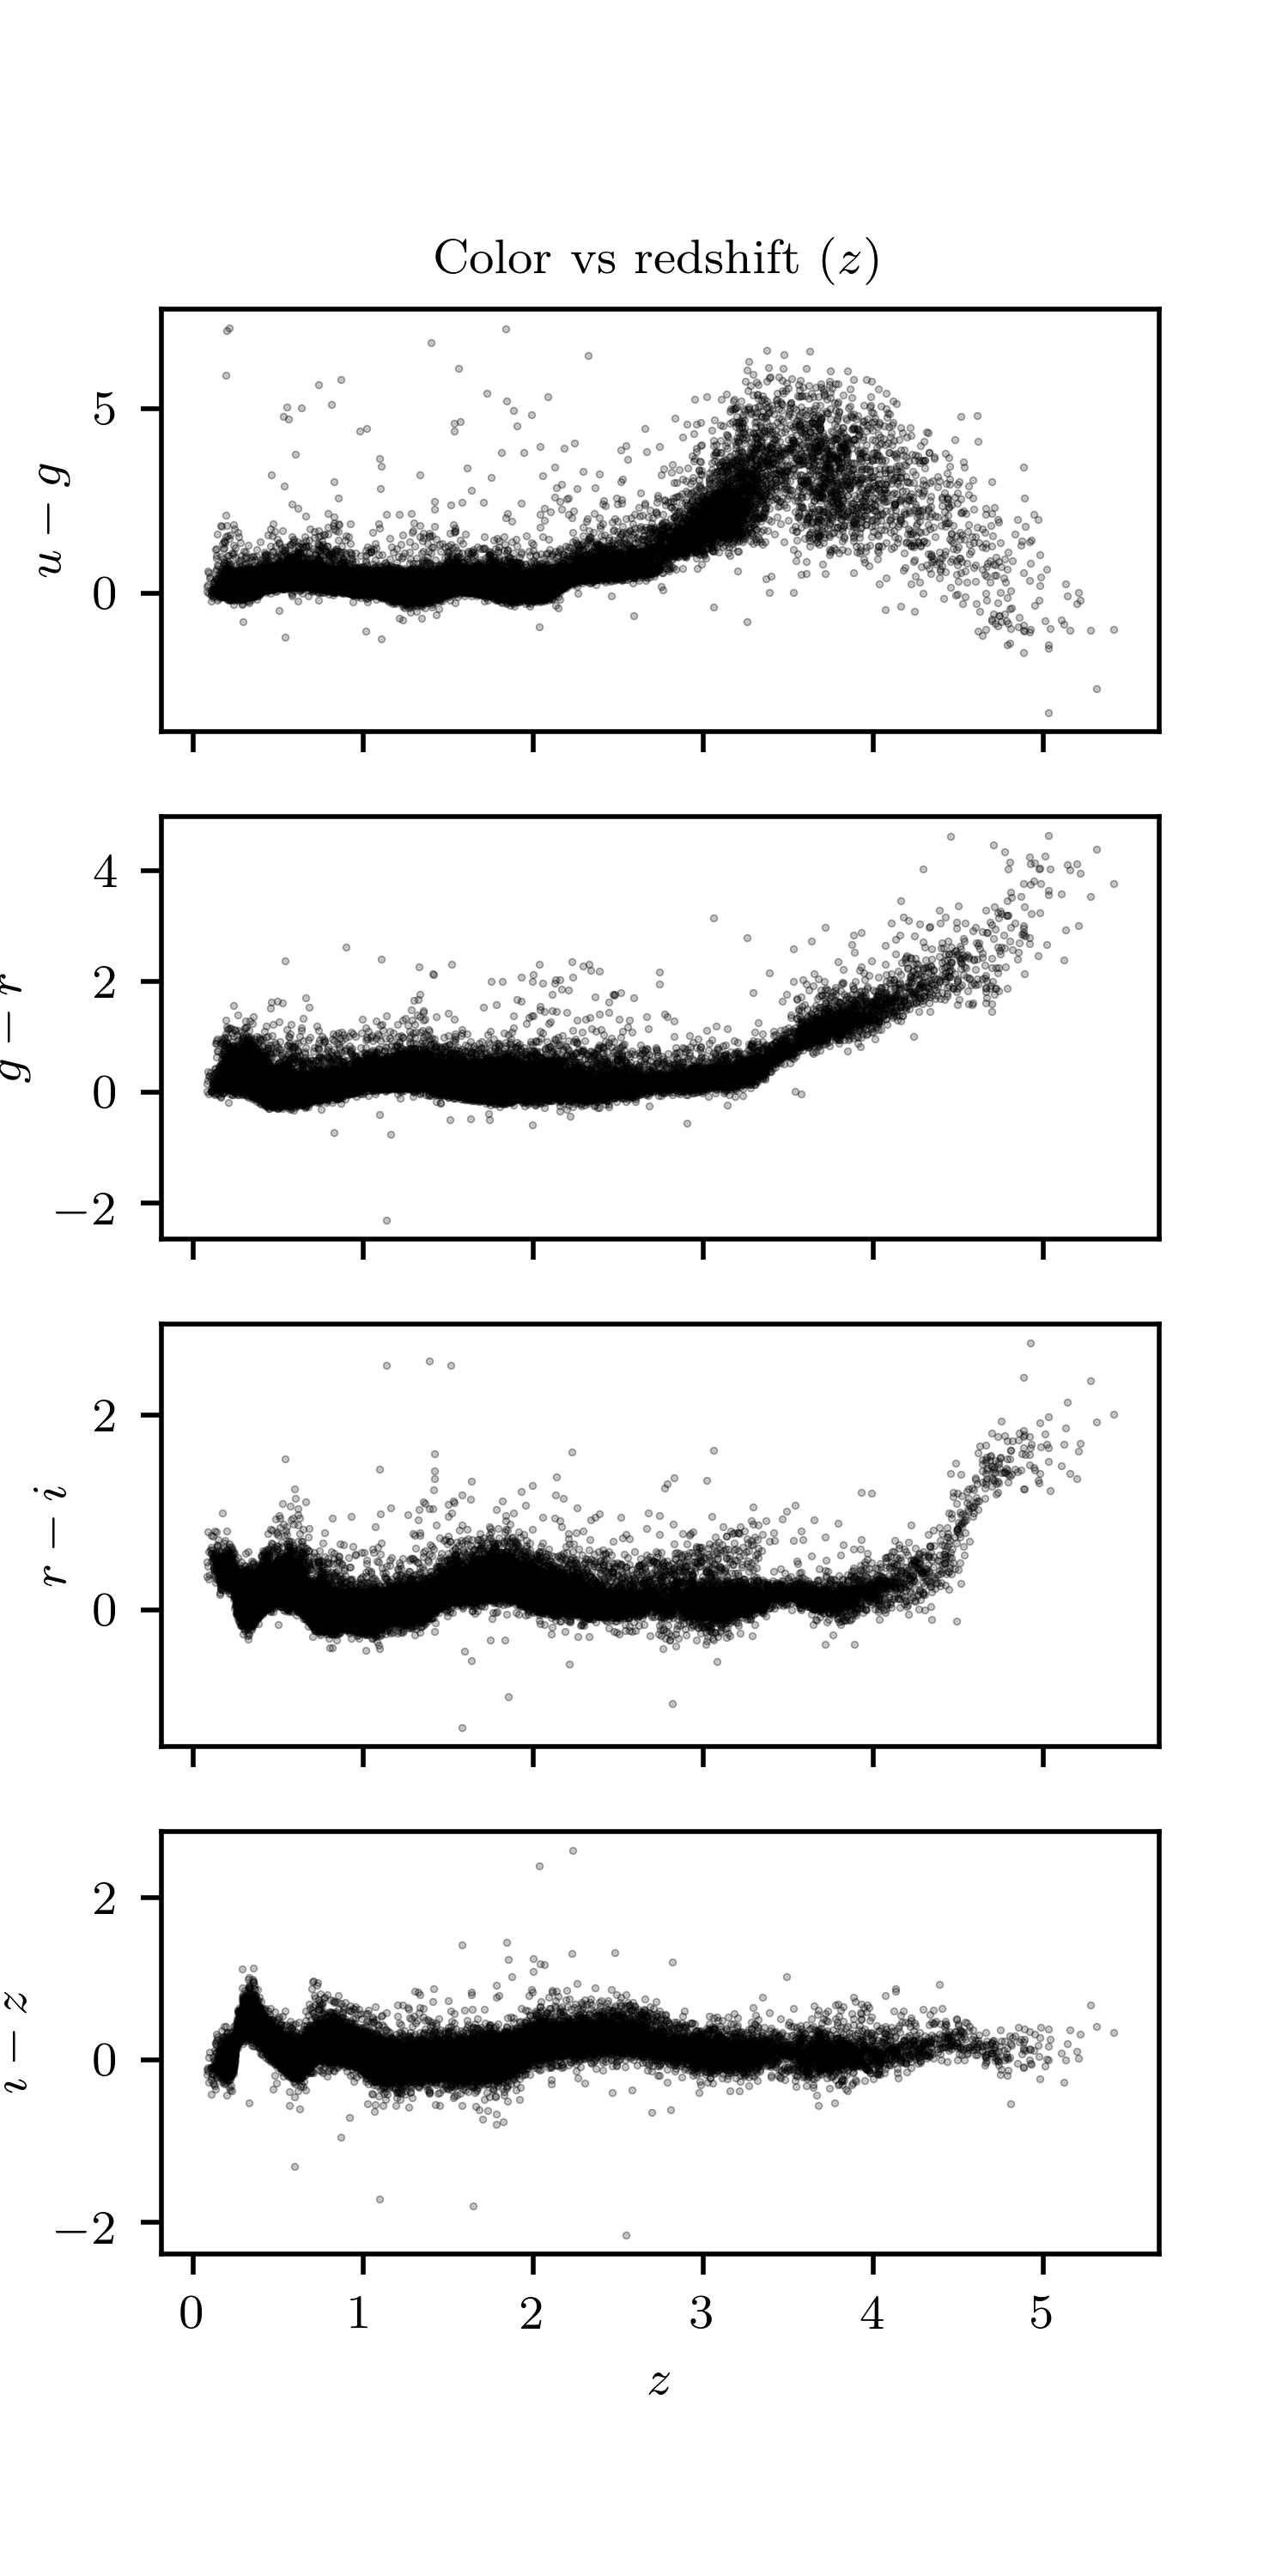
\includegraphics[width=\textwidth]{color-redshift}
	\caption{Color vs redshift plots for four different color bands ($u-g$, $g-r$, $r-i$, and $i-z$). For the sake of brevity, we will only find a regression for one of these relations, namely $r-i$ vs $z$.}
	\label{fig:color-redshift}
\end{figure}

We fit polynomials of degree $0$ through $15$ to our data, and find the $\chi^2$, Adjusted $R^2$, Akaike and Bayesian Information Criterions for each. Figure~\ref{fig:reg-err} shows these values by degree. For $\chi^2$, AIC, and BIC, lower is better, while we want a high adjusted $R^2$ value.
\begin{figure}
	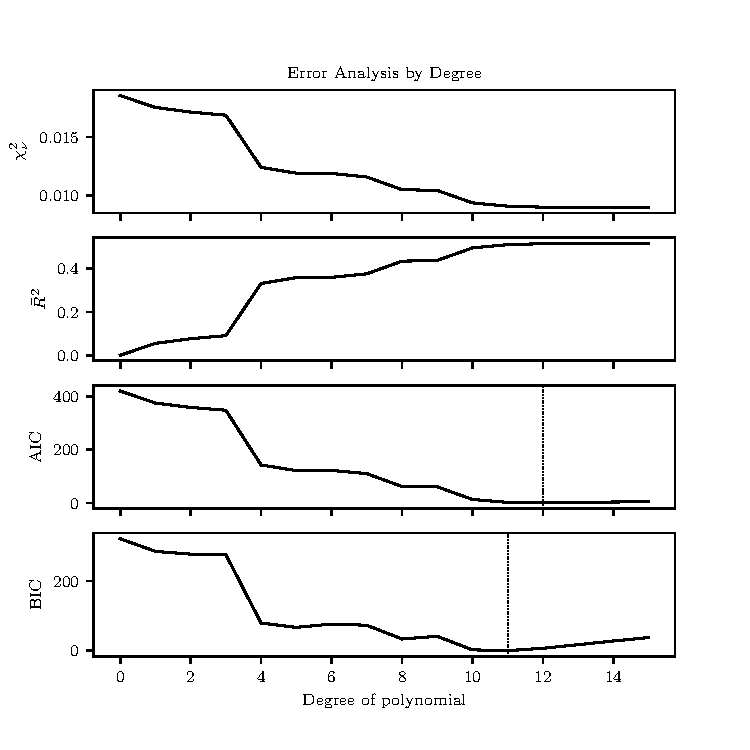
\includegraphics[width=\textwidth]{reg-err}
	\caption{Residual analysis and information criterion plots for polynomial regressions of degree $d$. The vertical lines at $d = 12$ and $d = 11$ represent the degrees which minimize the Akaike and Bayesian Information Criterion's respectively, indicating the polynomials which best fit the data without overfitting the data.}
	\label{fig:reg-err}
\end{figure}

We can also use cross validation to test how well polynomials of a certain degree predict the data when fitted to only a subset of it. We preform cross validation by randomly splitting our $r - i$ band measurements into a training set and cross validation set, and fitting a polynomial to the training data, and then calculating the $\chi^2$ value for the training and cross-validation data separately.
\begin{figure}
	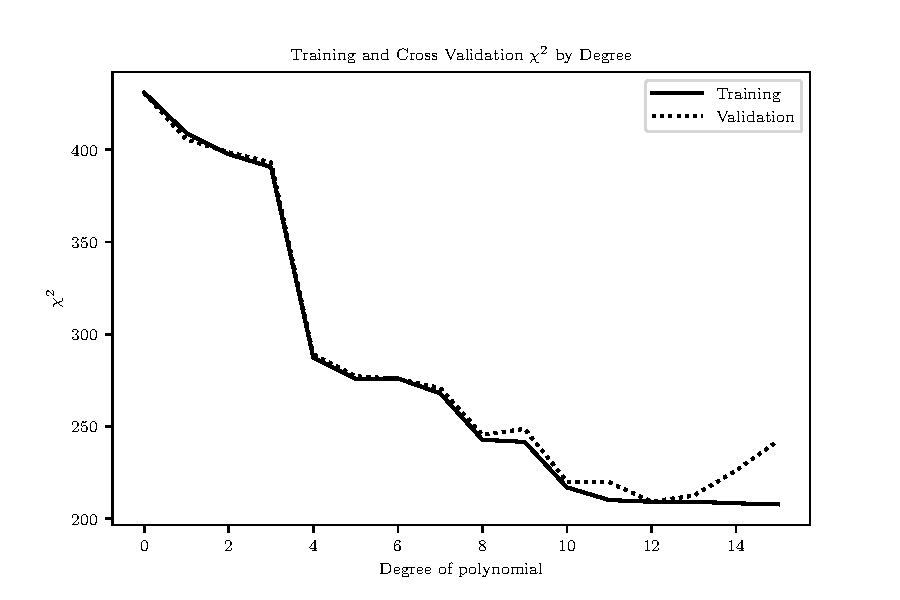
\includegraphics[width=\textwidth]{cross-val}
	\caption{Cross validation of polynomial fit by degree. Notice that for $d > 13$, the $\chi^2$ value begins to start increasing, indicating that past this point our regressions no longer adequately serve as predictors for the cross validation subset.}
	\label{fig:cross-val}
\end{figure}
Notice in Figure~\ref{fig:cross-val} that $\chi^2$ is minimized for the training data for all $d \geq 11$, while $\chi^2$ is minimized for the testing data for $d = 12,13$. After this point, we see a noticible uptick in the $\chi^2$ value, indicating that for degrees greater than $12$, the polynomial regressions no longer predict random subsamplings of our data better. This tells us that a degree of $11$, $12$ or $13$ is best suited to our data. To visualize our optimal regressions, we plot the polynomials of best fit, overlaying the data points in Figure~\ref{fig:best-reg}.

\begin{figure}
	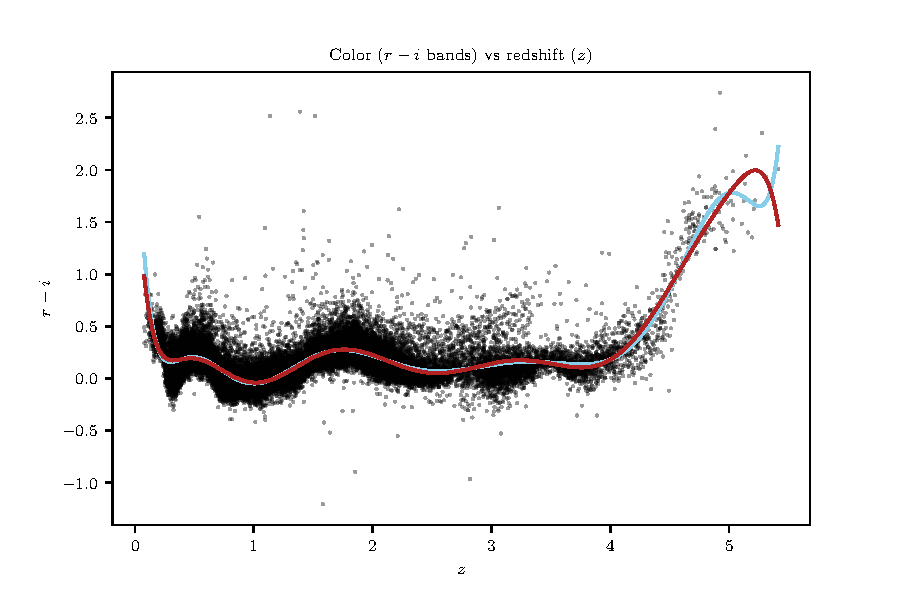
\includegraphics[width=\textwidth]{ri-redshift-deg}
	\caption{Polynomial regressions of degree $11$ (red) and $12$ (blue) for $r - i$ vs $z$. These polynomials are those which minimize the AIC and BIC.}
	\label{fig:best-reg}
\end{figure}
Both the $11$ and $12$ degree polynomials are similar to the results found by~\citeauthor{wu2003} in 2004, although the exact polynomials are not listed in their paper.
